\documentclass{standalone}
\begin{document}
\section{U-Net}
The U-net is a convolutional network architecture for fast and precise segmentation of images especially in the biomedical field\cite{unet}.
One of the main advantage of the U-net is the ability of dealing with small dataset. The name U-net refers to the U shape of the network architecture. 
The whole structure is divided into two main parts, as shown in Figure\ref{fig:unet}:

\paragraph{Encoder}:
or contraction path is a sequence of convolutional and max pooling layers with the aim of extracting features and reducing dimensionality.

\paragraph{Decoder}:
or expansion path is a sequence of transpose convolutional layers to with the aim of reconstruct the feature map and consequently the segmentation mask.
\begin{figure}[htp]

    \centering
    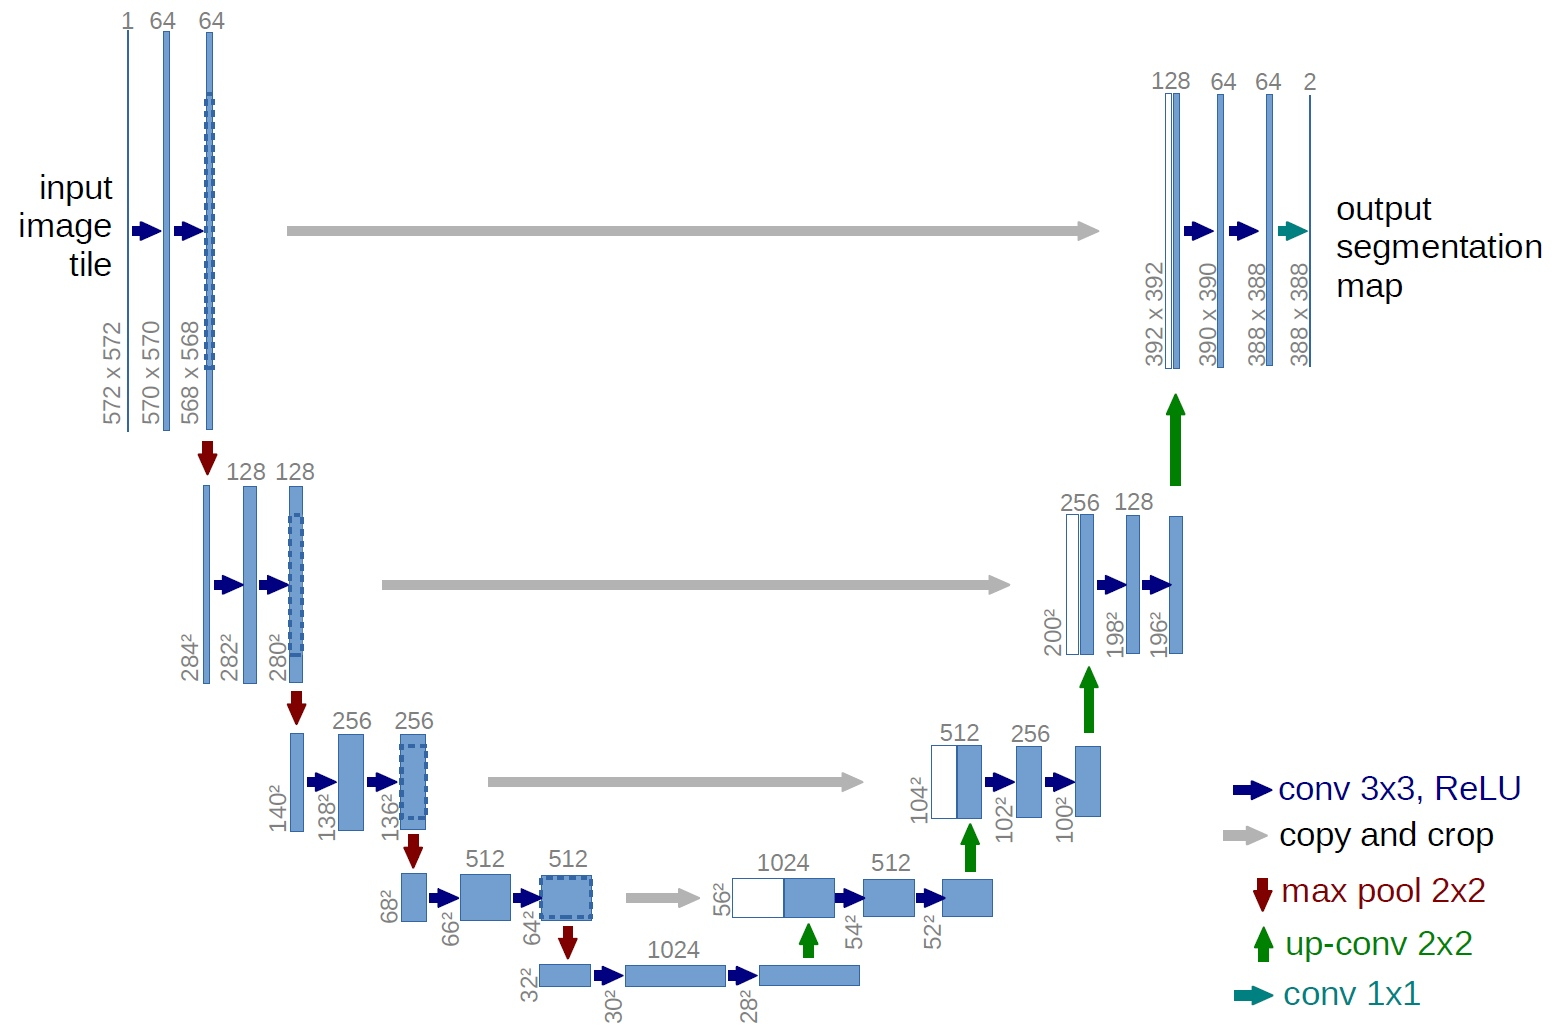
\includegraphics[width=.9\textwidth]{../images/U-Net arch.jpeg}
    
    \caption{Original U-Net architecture. From\cite{unet}}
    \label{fig:unet}
    
    \end{figure}
\\
The \textit{Encoder} is a typical Convolutional Neural Network that consists in the repeated application of convolutions, followed by ReLu activation function and max pooling operations.
During the contraction the input size is decreased and so the spatial information, while the information about features is increased.
The \textit{Decoder} combines the features extracted in the contraction path  with tha spatial information by a sequence of transpose convolutions (or up-convolutions) and concatenations (grey arrows in Figure\ref{fig:unet}).



\end{document}